\documentclass[11pt,letterpaper]{article}

\usepackage[margin=1in]{geometry}
\usepackage{lmodern}
\usepackage{amsmath,amssymb}
\usepackage{booktabs}
\usepackage{graphicx}
\usepackage{xcolor}
\usepackage{tabularx}
\usepackage{pifont}
\usepackage{colortbl}
\usepackage{tikz}
\usetikzlibrary{positioning, arrows.meta}
\usepackage[hyphens]{url}
\usepackage[round]{natbib}
\usepackage[font=small,labelfont=bf,skip=4pt]{caption}
\usepackage{hyperref}

\hypersetup{
    colorlinks=true,
    linkcolor=blue!70!black,
    citecolor=blue!70!black,
    urlcolor=blue!70!black
}

\setlength{\parindent}{1.5em}
\setlength{\parskip}{0.3em}

\setcounter{secnumdepth}{3}
\setcounter{tocdepth}{2}

\title{
    \vspace{-1.5em}
    {\LARGE\bfseries Supplementary Material for FinAbstain:}\\[0.3em]
    {\Large Do Small Open Language Models Know Why a Financial Question Cannot Be Answered?}
}

\author{
    \textbf{Kartik Sirohi}\textsuperscript{1}\thanks{Contact: \protect\url{https://sirohikartik.github.io}} \qquad
    \textbf{Kumar Prateek}\textsuperscript{1} \qquad
    \textbf{Simranjit Singh}\textsuperscript{1}\thanks{Corresponding author: \protect\url{singhsimranjit@nitj.ac.in}}\\[0.4em]
    \textsuperscript{1}Department of Information Technology,\\
    Dr.~B.~R.~Ambedkar National Institute of Technology Jalandhar, Punjab, 144008, India
}

\date{}

\begin{document}

\maketitle
\vspace{-1em}

\begin{abstract}
This document provides the complete supplementary material for the benchmark \textbf{FinAbstain}. It contains comprehensive dataset composition analyses, token-level and context distributions, financial fact type distributions, multi-judge automated validation funnels, full human evaluation protocols and confusion matrices, verbatim prompt templates, reproducibility specifications, and the official AI use statement.
\end{abstract}

\vspace{0.8em}
\hrule
\vspace{0.5em}
\tableofcontents
\vspace{0.8em}
\hrule
\vspace{1.5em}

\section{Dataset Composition and Analysis Methodology}
\label{app:dataset_analysis}

This section describes the composition of FinAbstain and the empirical procedures used to analyze its categories, token lengths, fact types, source reports, target positions, and validation process. The final benchmark contains 143 verified samples drawn from FY2024 corporate financial reports.

\subsection{Taxonomy and Decision Distribution}
\label{app:taxonomy}

The benchmark contains 143 samples evaluated at two levels of decision granularity. The primary level is the binary gold decision (\textit{Answer} vs.\ \textit{Abstain}). The secondary level comprises four mutually exclusive, fine-grained operational categories: \textit{Answerable}, \textit{Conflict}, \textit{Missing}, and \textit{Ambiguous}.

\begin{table}[h]
\centering
\small
\caption{Dataset category distribution across the 143 benchmark samples.}
\label{tab:category_distribution}
\begin{tabular}{lrr}
\toprule
\textbf{Category} & \textbf{Count} & \textbf{Percentage} \\
\midrule
Answerable & 50 & 35.0\% \\
Conflict   & 38 & 26.6\% \\
Missing    & 33 & 23.1\% \\
Ambiguous  & 22 & 15.4\% \\
\midrule
\textbf{Total} & \textbf{143} & \textbf{100.0\%} \\
\bottomrule
\end{tabular}
\end{table}

The \textbf{Answerable} category contains samples where the target financial fact is uniquely and unambiguously present in the context. \textbf{Conflict} samples contain multiple contradictory values for the exact same target fact. \textbf{Missing} samples concern a target topic where the specific queried metric has been excised. \textbf{Ambiguous} samples contain questions with underspecified reporting dimensions (such as fiscal period, reporting unit, or operating segment).

\begin{table}[h]
\centering
\small
\caption{Gold decision distribution across the 143 benchmark samples.}
\label{tab:gold_decision_distribution}
\begin{tabular}{lrr}
\toprule
\textbf{Decision} & \textbf{Count} & \textbf{Percentage} \\
\midrule
Answer  & 50 & 35.0\% \\
Abstain & 93 & 65.0\% \\
\midrule
\textbf{Total} & \textbf{143} & \textbf{100.0\%} \\
\bottomrule
\end{tabular}
\end{table}

The fine-grained category and binary decision distributions are illustrated together as a nested ring chart in Figure~\ref{fig:category_distribution}.

\begin{figure}[h]
    \centering
    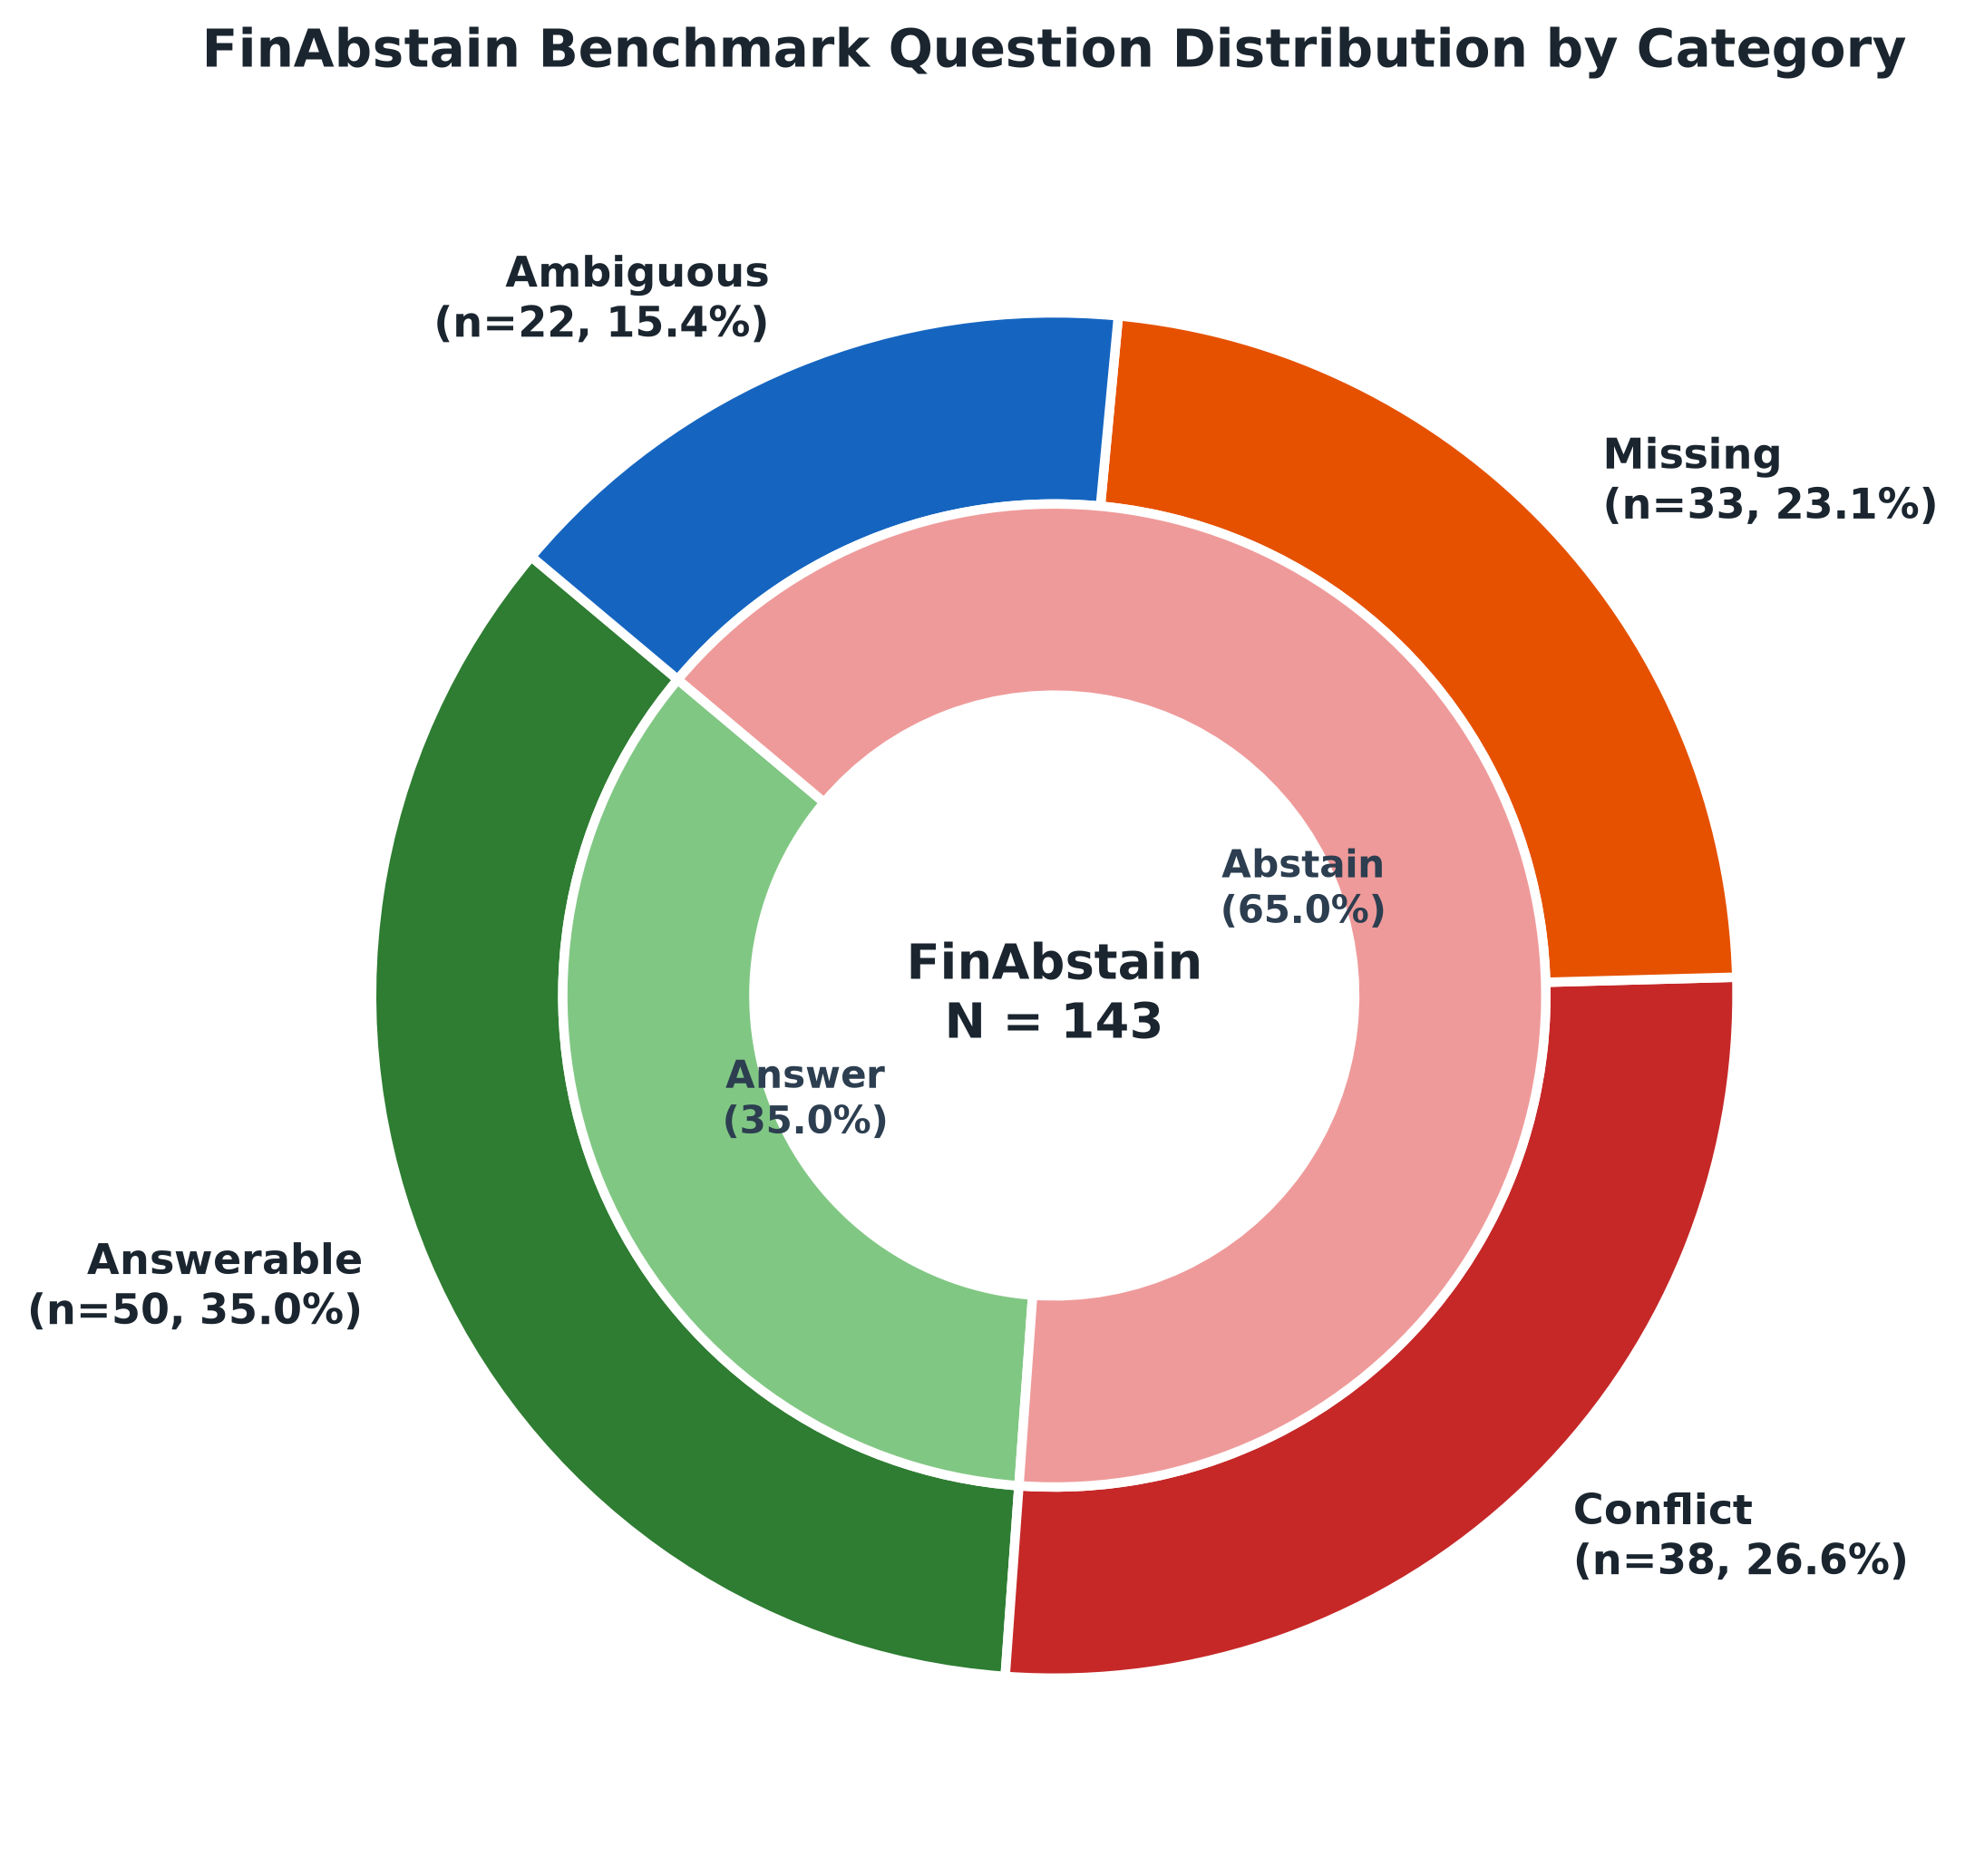
\includegraphics[width=0.55\textwidth]{figures/fig1_category_distribution_donut.png}
    \caption{Gold decision (inner ring) and fine-grained category (outer ring) distributions across FinAbstain.}
    \label{fig:category_distribution}
\end{figure}

\subsection{Tokenization and Length Statistics}
\label{app:token_analysis}

Token lengths were measured using OpenAI's \texttt{cl100k\_base} Byte-Pair Encoding (BPE) tokenizer via the \texttt{tiktoken} library. For each sample $i \in \{1,\ldots,N\}$, token lengths were recorded for the question, short target context, full context, evidence span, and original answer. Table~\ref{tab:token_statistics} reports descriptive statistics across these fields.

\begin{table*}[t]
\centering
\small
\caption{Token-level statistics across the 143 samples (using the \texttt{cl100k\_base} tokenizer).}
\label{tab:token_statistics}
\begin{tabular}{lrrrrr}
\toprule
\textbf{Field} & \textbf{Mean} & \textbf{Std.} & \textbf{Median} & \textbf{Min} & \textbf{Max} \\
\midrule
Question                            & 21.17   & 5.67   & 22.0   & 8    & 35   \\
Short context (target passage)      & 763.26  & 159.96 & 745.0  & 357  & 1226 \\
Full context (padded filing text)   & 7668.29 & 255.15 & 7693.0 & 6963 & 8177 \\
Evidence span                       & 32.52   & 23.25  & 26.0   & 6    & 151  \\
Original answer (pre-edit, $N=143$) & 4.38    & 2.08   & 5.0    & 1    & 23   \\
Gold answer (answerable only, $N=50$)& 3.98   & 1.46   & 4.0    & 1    & 7    \\
\bottomrule
\end{tabular}
\end{table*}

\begin{figure}[h]
    \centering
    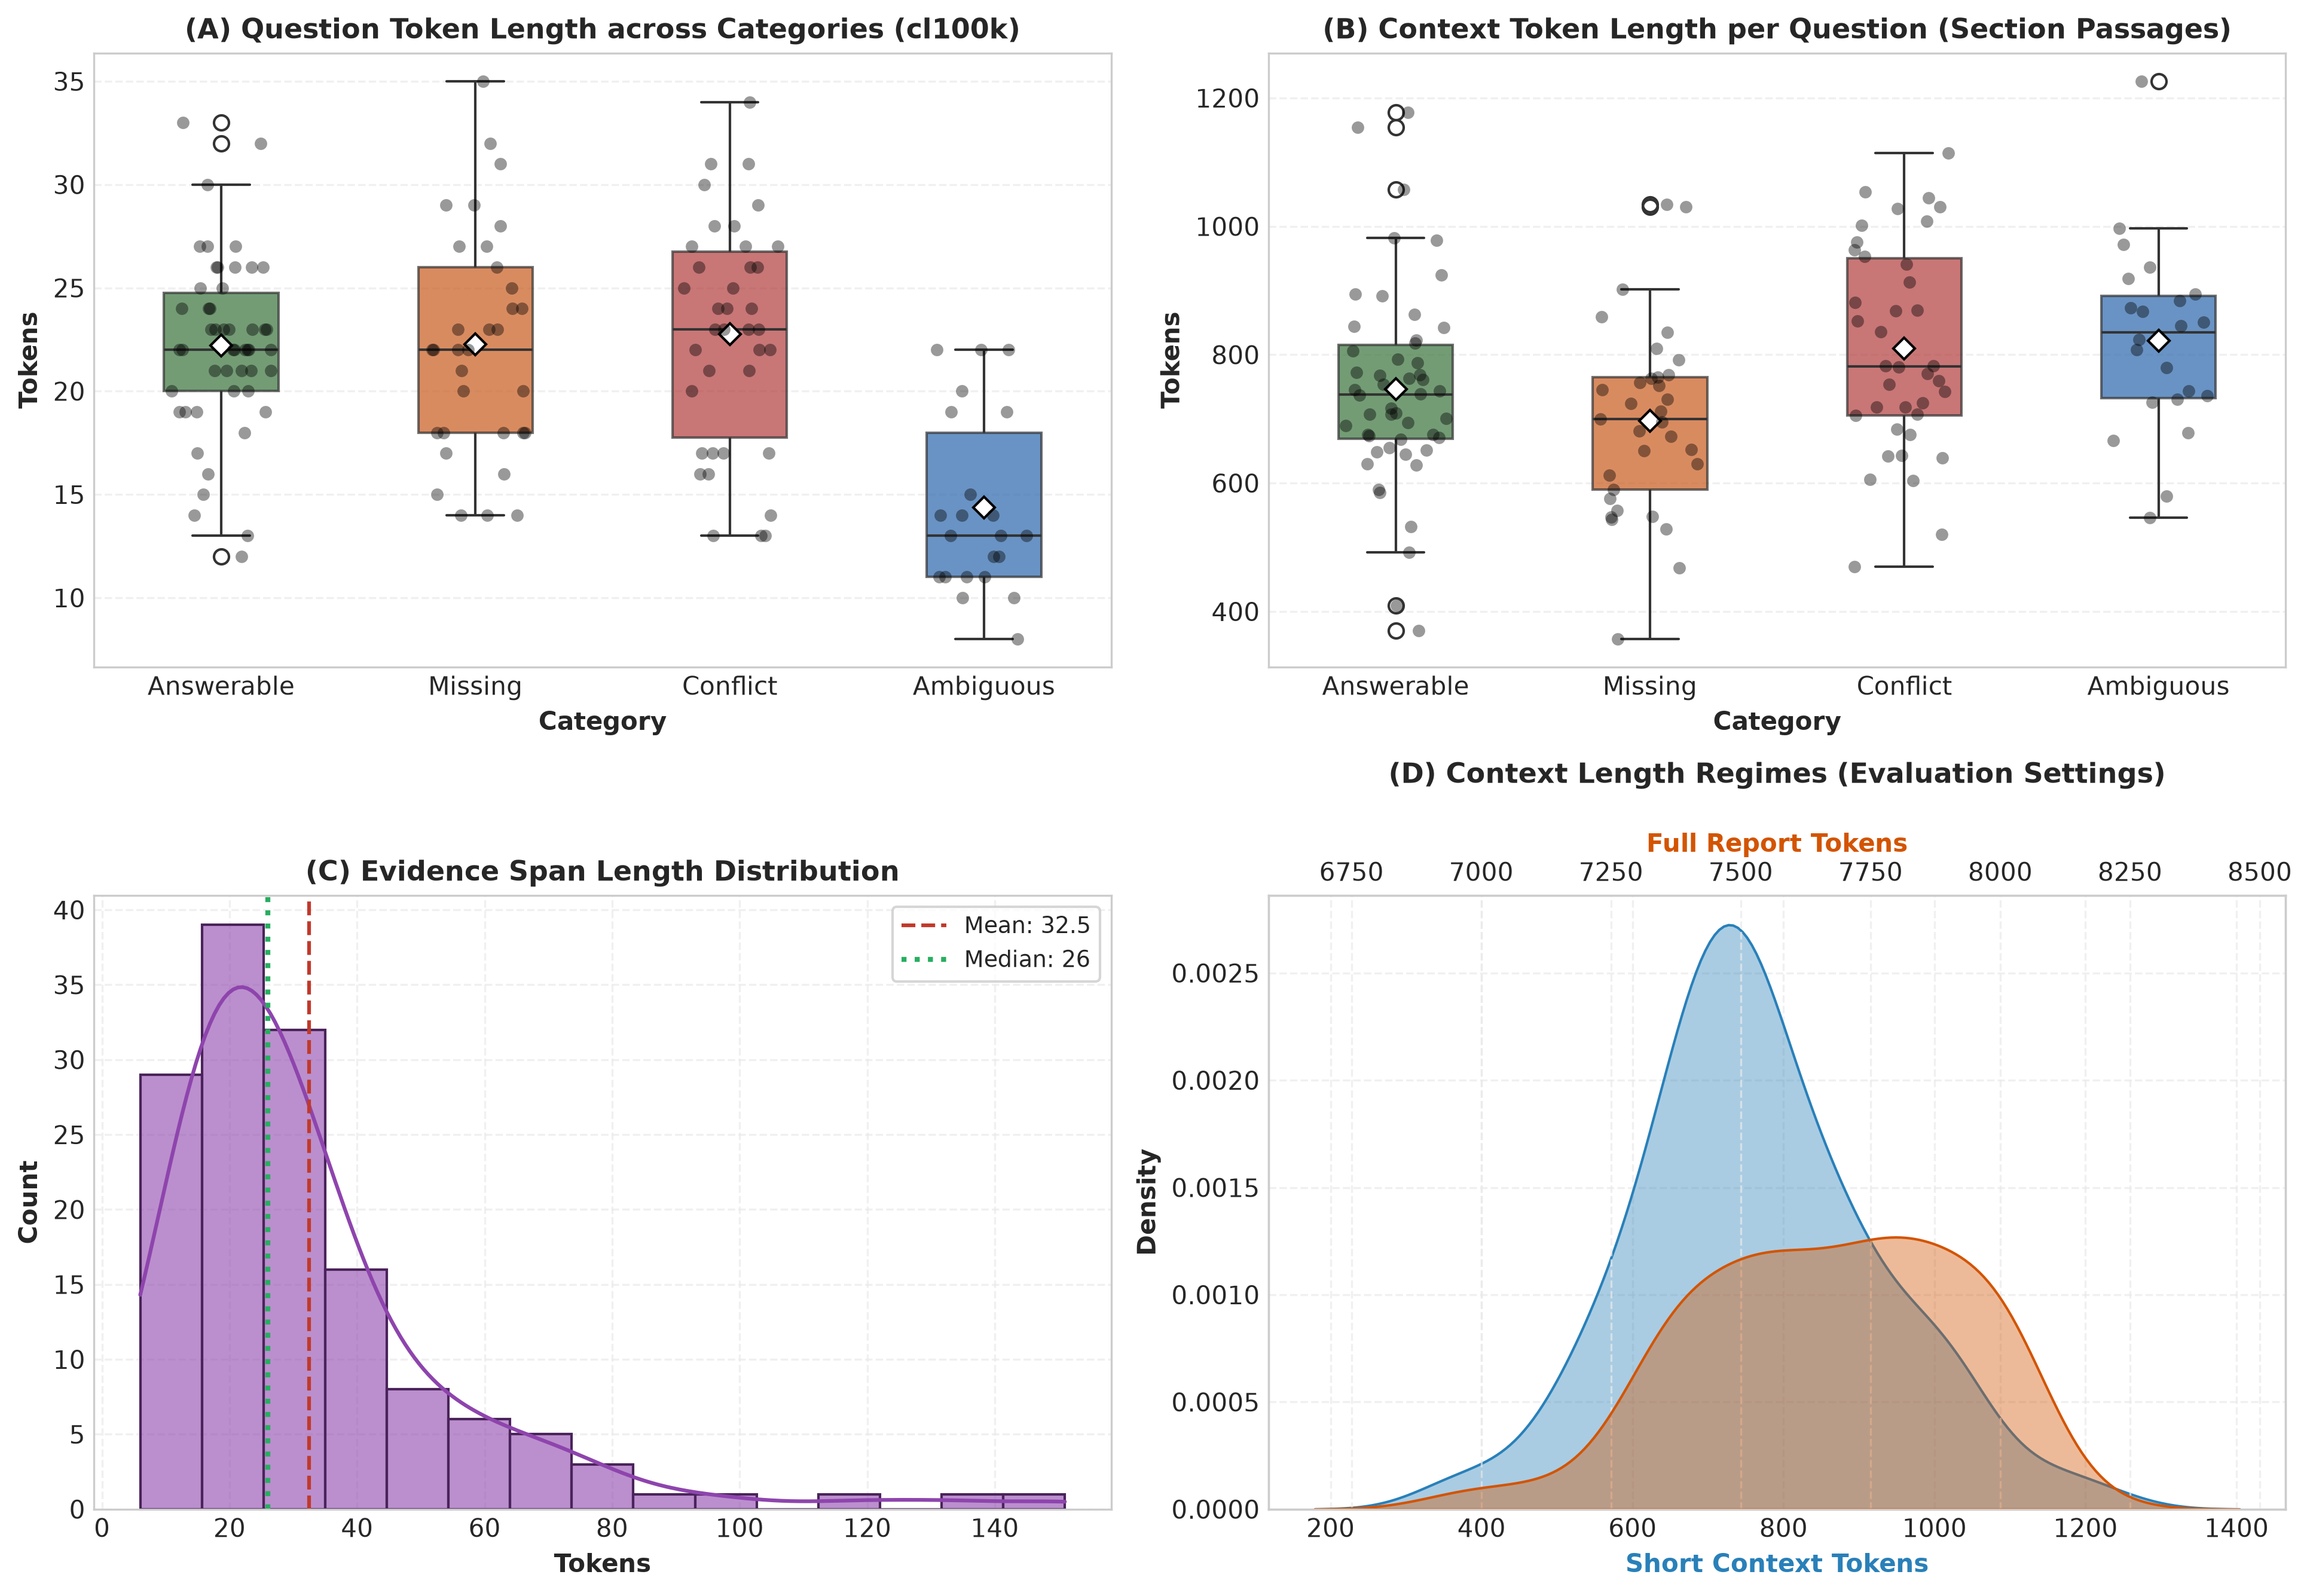
\includegraphics[width=0.7\textwidth]{figures/fig3_token_length_distributions.png}
    \caption{Token-length distributions for questions, short contexts, and evidence spans across categories.}
    \label{fig:token_distributions}
\end{figure}

\subsubsection{Context Length Analysis by Category}
Short-context lengths were inspected across fine-grained categories to verify that label assignment did not introduce significant passage-length bias. Table~\ref{tab:category_context_lengths} shows the category-level means.

\begin{table}[h]
\centering
\small
\caption{Short-context length broken down by benchmark category.}
\label{tab:category_context_lengths}
\begin{tabular}{lr}
\toprule
\textbf{Category} & \textbf{Mean Tokens} \\
\midrule
Answerable & 746.3 \\
Conflict   & 809.6 \\
Missing    & 696.6 \\
Ambiguous  & 822.0 \\
\bottomrule
\end{tabular}
\end{table}

\subsection{Financial Fact Types and Source Reports}
\label{app:fact_types}

Each question--evidence pair was classified by its target fact type across six categories: Amount, Date, Percentage, Name, Count, and Other (Table~\ref{tab:fact_types}).

\begin{table}[h]
\centering
\small
\caption{Distribution of financial fact types.}
\label{tab:fact_types}
\begin{tabular}{lrr}
\toprule
\textbf{Fact type} & \textbf{Count} & \textbf{Percentage} \\
\midrule
Amount     & 94  & 65.7\% \\
Date       & 18  & 12.6\% \\
Percentage & 13  & 9.1\%  \\
Name       & 10  & 7.0\%  \\
Count      & 5   & 3.5\%  \\
Other      & 3   & 2.1\%  \\
\midrule
\textbf{Total} & \textbf{143} & \textbf{100.0\%} \\
\bottomrule
\end{tabular}
\end{table}

The benchmark items are grounded in four corporate SEC 10-K filings from fiscal year 2024, representing distinct business sectors (Table~\ref{tab:source_reports}).

\begin{table}[h]
\centering
\small
\caption{Distribution of benchmark source reports.}
\label{tab:source_reports}
\begin{tabular}{lrr}
\toprule
\textbf{Source report} & \textbf{Count} & \textbf{Percentage} \\
\midrule
Pfizer (Healthcare)        & 52 & 36.4\% \\
Coca-Cola (Beverages)      & 42 & 29.4\% \\
Caterpillar (Industrial)   & 32 & 22.4\% \\
Amazon (Retail / Tech)     & 17 & 11.9\% \\
\midrule
\textbf{Total} & \textbf{143} & \textbf{100.0\%} \\
\bottomrule
\end{tabular}
\end{table}

Figure~\ref{fig:fact_reports} summarizes the fact-type and source-report distributions.

\begin{figure}[h]
    \centering
    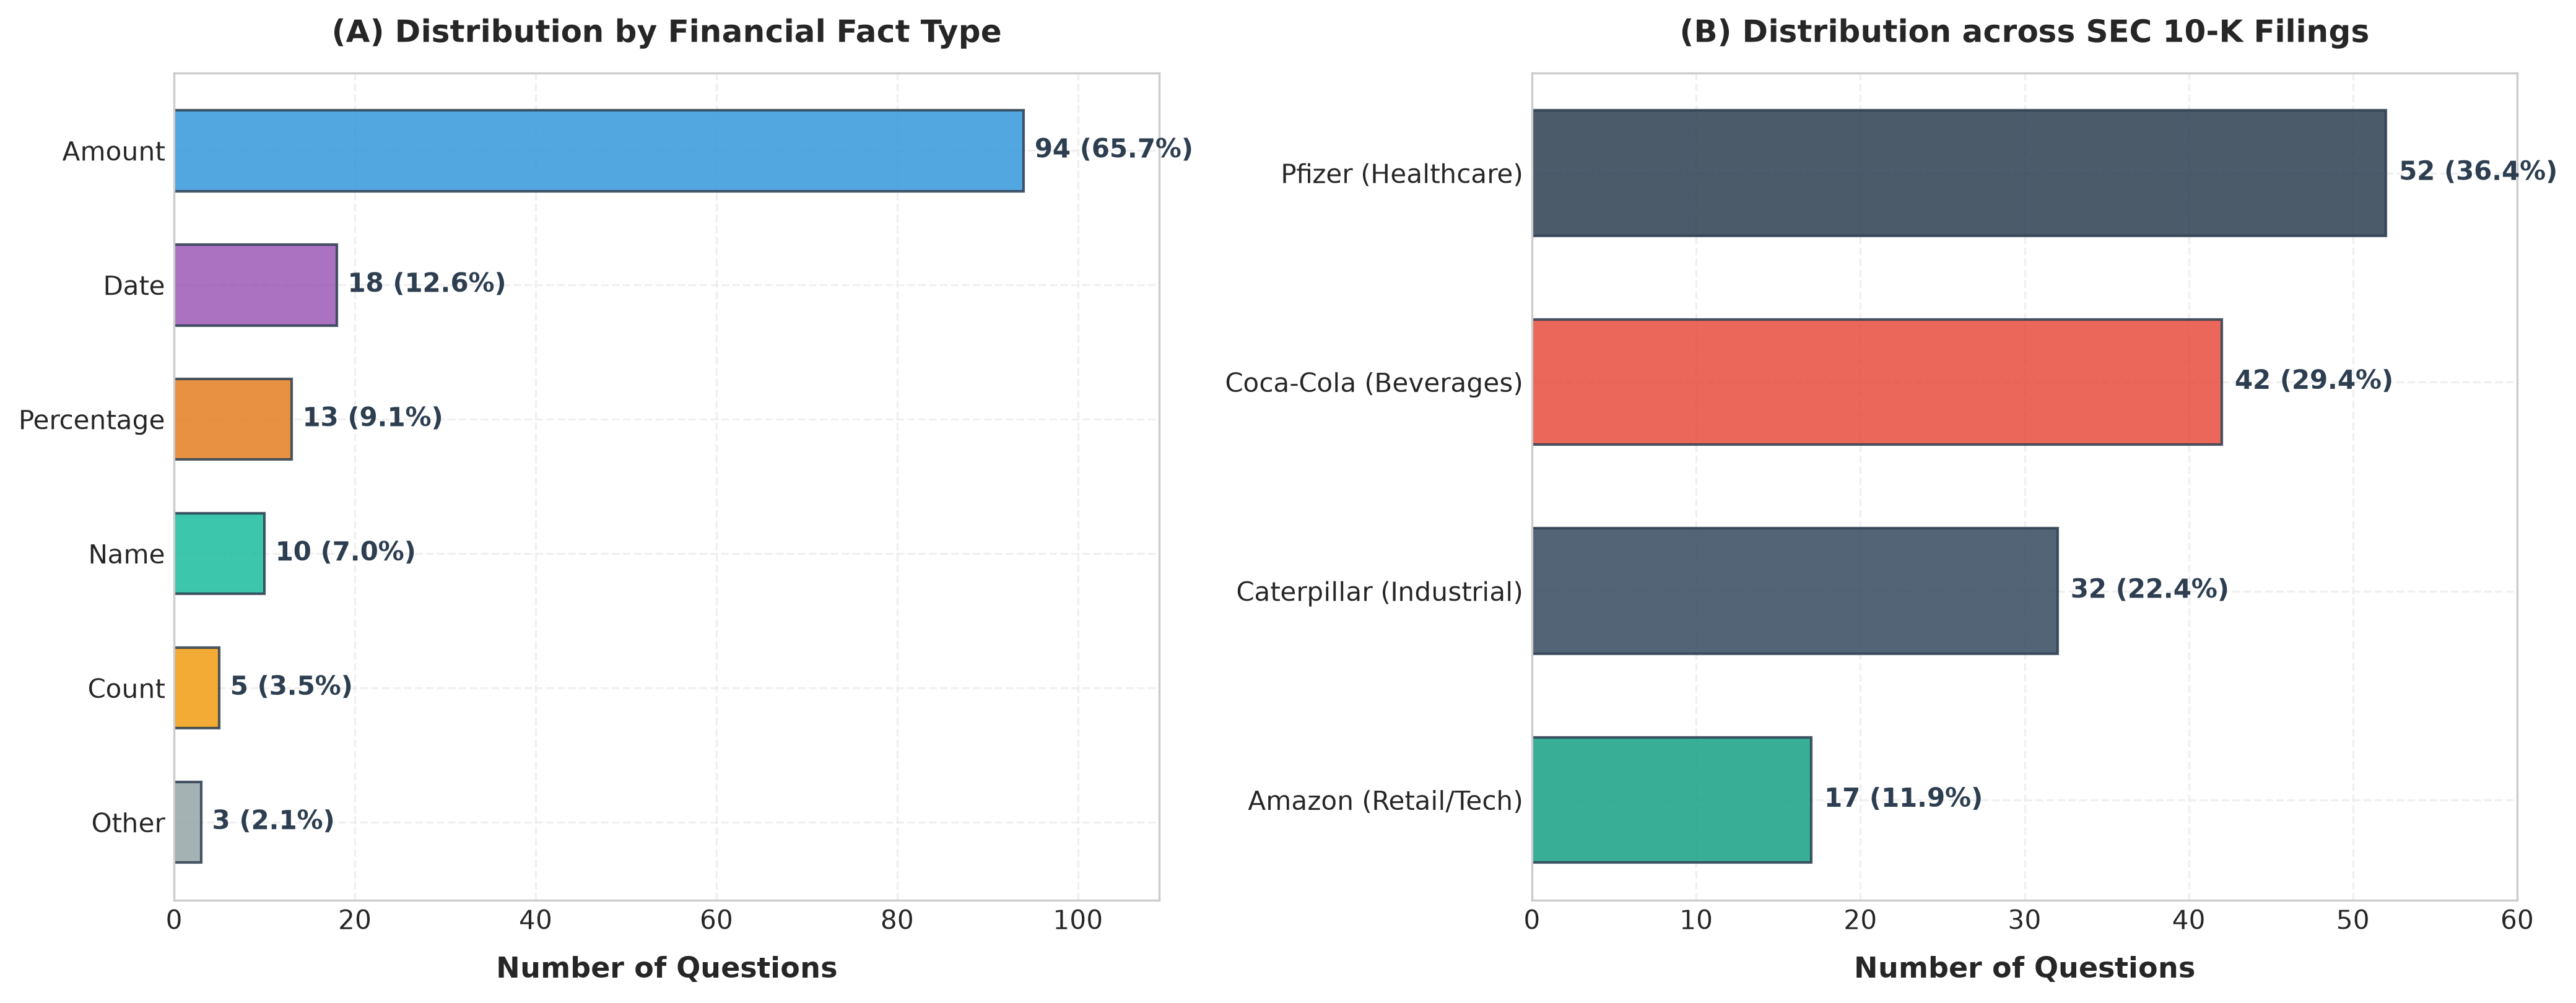
\includegraphics[width=0.7\textwidth]{figures/fig2_fact_types_and_reports.png}
    \caption{Frequency breakdown of financial fact types and corporate source filings.}
    \label{fig:fact_reports}
\end{figure}

\subsection{Question Type Distribution}
\label{app:question_types}

Questions were categorized by their syntactic interrogative form: \textit{What}, \textit{Other}, \textit{How much/many}, and \textit{Which} (Table~\ref{tab:question_types}).

\begin{table}[h]
\centering
\small
\caption{Question type distribution in FinAbstain.}
\label{tab:question_types}
\begin{tabular}{lrr}
\toprule
\textbf{Question type} & \textbf{Count} & \textbf{Percentage} \\
\midrule
What          & 106 & 74.1\% \\
Other         & 25  & 17.5\% \\
How much/many & 7   & 4.9\%  \\
Which         & 5   & 3.5\%  \\
\midrule
\textbf{Total} & \textbf{143} & \textbf{100.0\%} \\
\bottomrule
\end{tabular}
\end{table}

\subsection{Normalized Target Position Depth}
\label{app:target_position}

Each benchmark item places the target evidence section at a normalized context depth $\tau_i \in [0.0, 1.0]$, defined as:
\begin{equation}
\tau_i = \frac{\text{target\_section\_index}_i}{\max(N_{\text{sections}}-1, 1)}.
\label{eq:target_position}
\end{equation}
Here $\tau_i = 0.0$ corresponds to the absolute beginning of the context and $\tau_i = 1.0$ corresponds to the end.

\begin{table}[h]
\centering
\small
\caption{Normalized target position depth statistics.}
\label{tab:target_position}
\begin{tabular}{lr}
\toprule
\textbf{Statistic} & \textbf{Value} \\
\midrule
Mean               & 0.469 \\
Standard deviation & 0.311 \\
Median             & 0.444 \\
Minimum            & 0.000 \\
Maximum            & 1.000 \\
\bottomrule
\end{tabular}
\end{table}

Figure~\ref{fig:target_position} visualizes the distribution of target positions, confirming that target evidence is uniformly dispersed throughout the 8,000-token contexts rather than clustered at boundaries.

\begin{figure}[h]
    \centering
    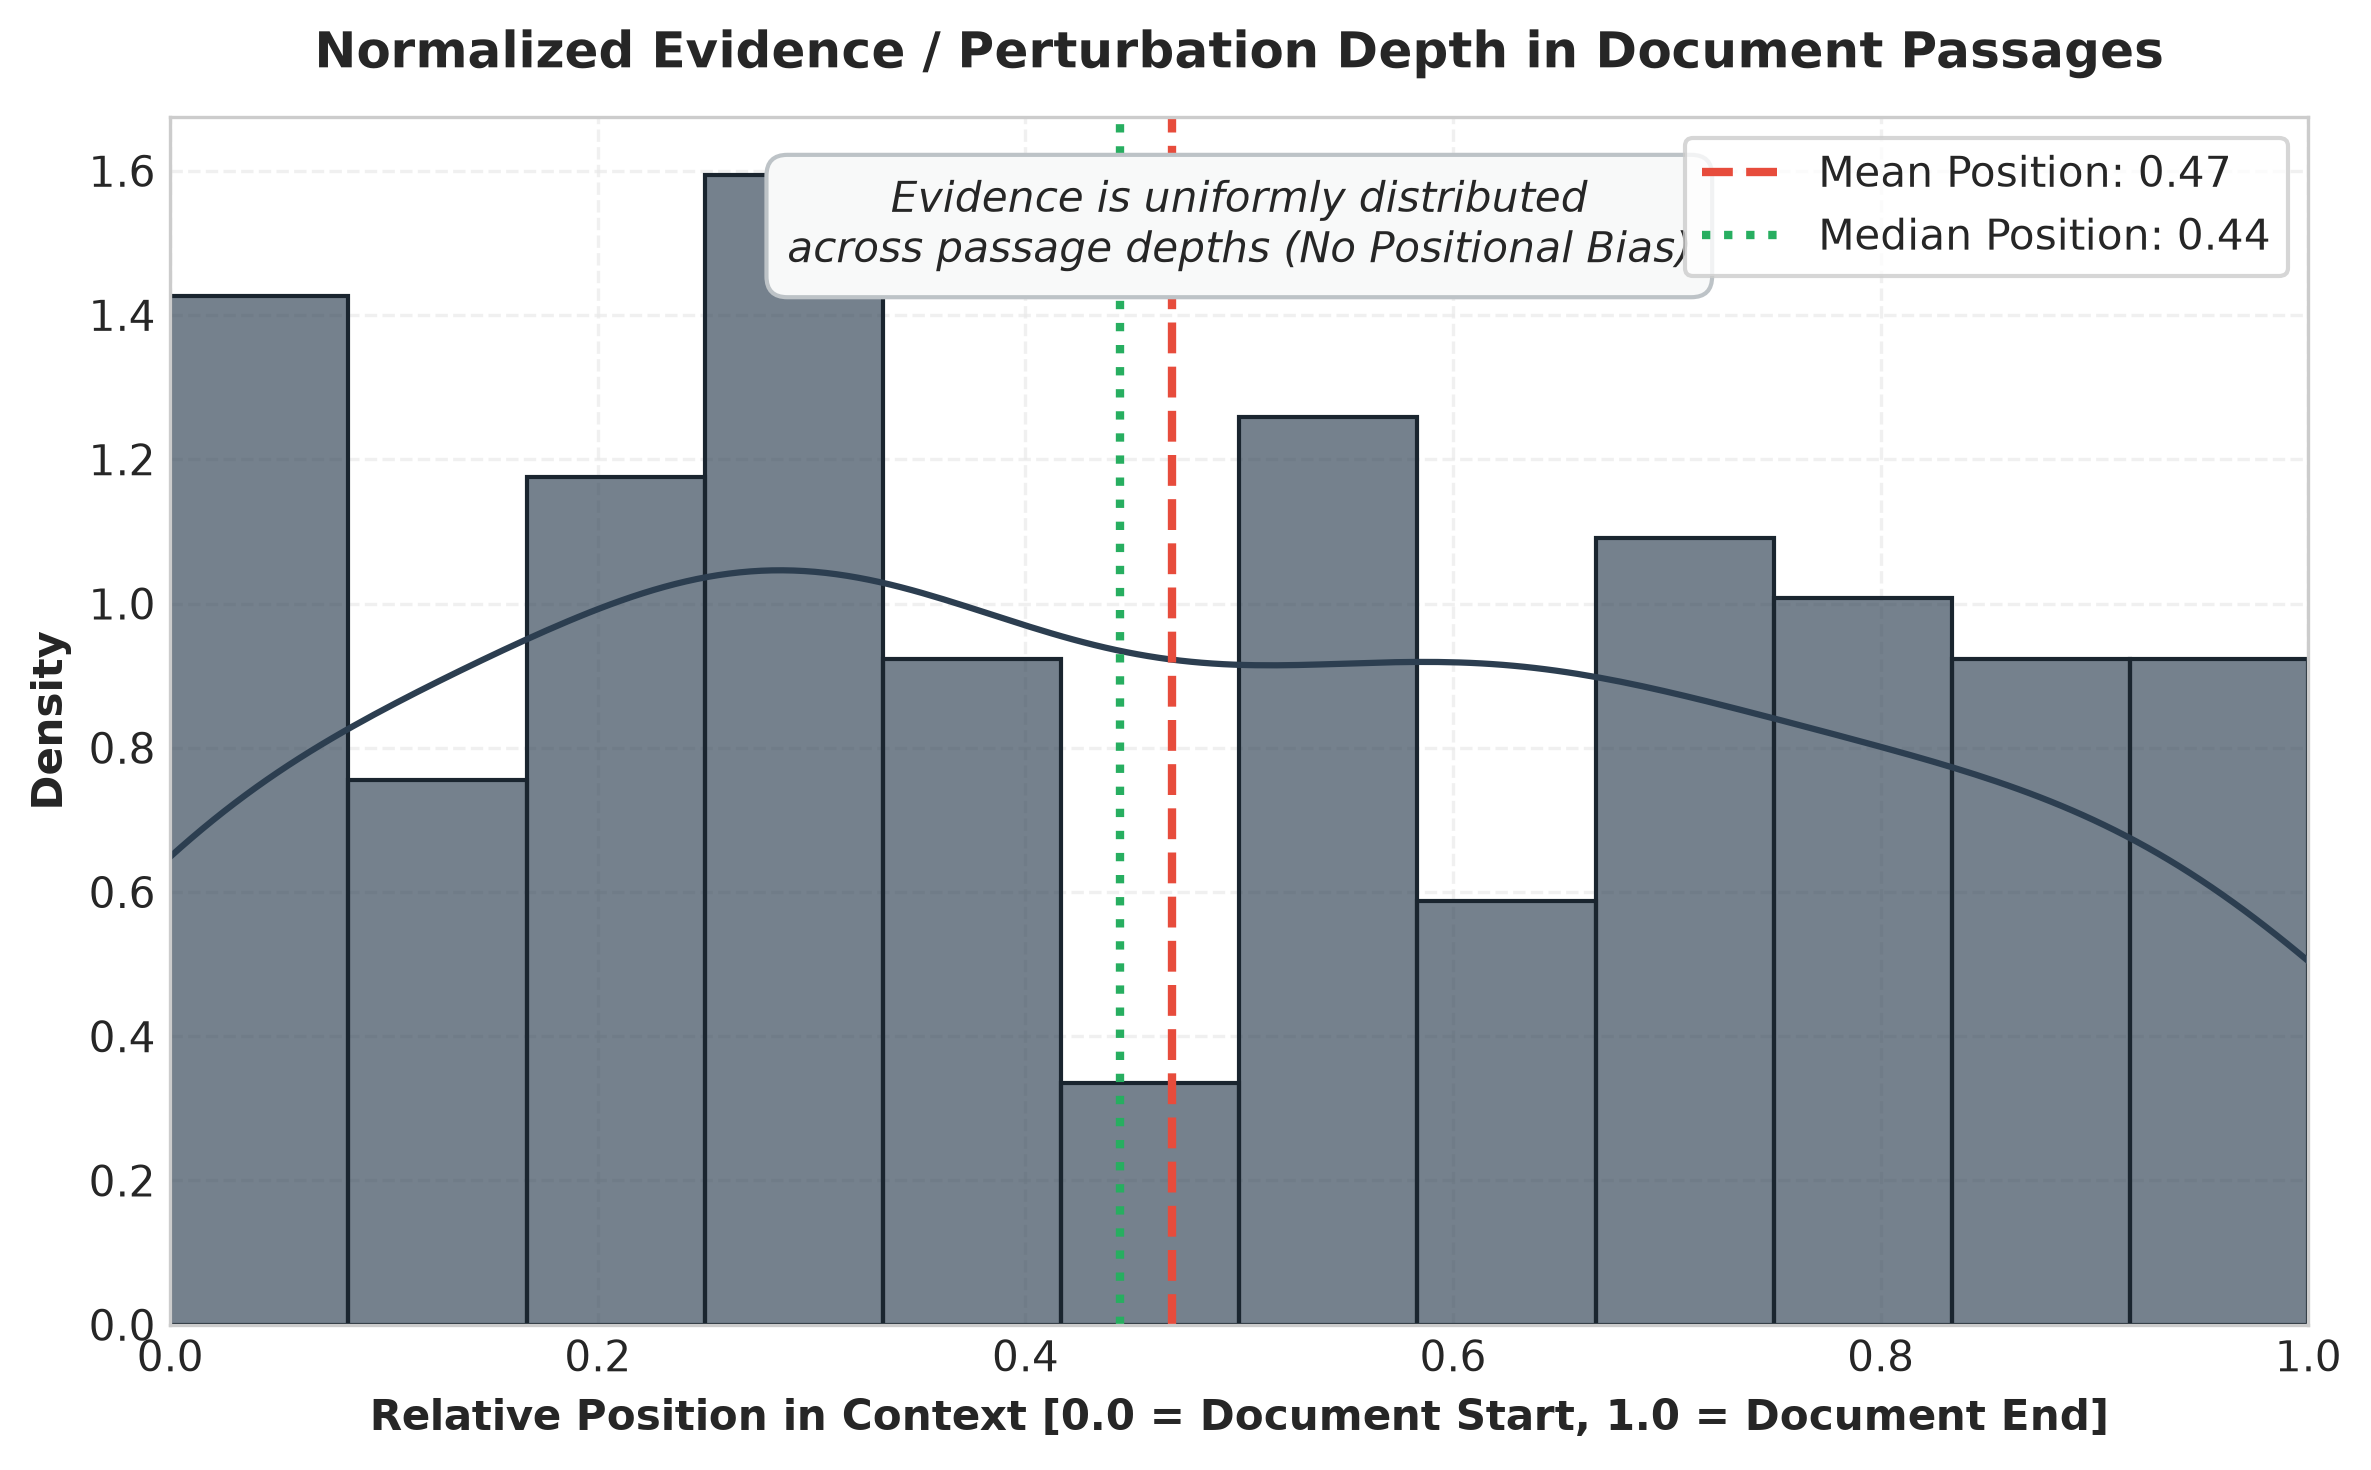
\includegraphics[width=0.65\textwidth]{figures/fig4_target_position_depth.png}
    \caption{Empirical distribution and Gaussian kernel density estimate of normalized target position depth.}
    \label{fig:target_position}
\end{figure}

\subsection{Multi-Judge Automated Validation Funnel}
\label{app:validation}

All candidate perturbations were subjected to strict automated verification before benchmark inclusion. Two independent models served as blind validators: \texttt{gpt-oss:120b} (Validator A) and \texttt{nemotron-3-super} (Validator B). Neither validator had access to the gold category label, edit metadata, or ground-truth answer. An item was accepted only if both models agreed exactly with the intended category.

Across 183 evaluated candidate items, 143 passed both validators ($78.1\%$) and 40 were rejected ($21.9\%$), as summarized in Table~\ref{tab:validation_funnel} and Figure~\ref{fig:validation_funnel}.

\begin{table}[h]
\centering
\small
\caption{Automated multi-judge validation funnel.}
\label{tab:validation_funnel}
\begin{tabular}{lrr}
\toprule
\textbf{Stage} & \textbf{Count} & \textbf{Percentage} \\
\midrule
Candidate items evaluated & 183 & 100.0\% \\
Accepted into benchmark   & 143 & 78.1\%  \\
Rejected                  & 40  & 21.9\%  \\
\bottomrule
\end{tabular}
\end{table}

\begin{figure}[h]
    \centering
    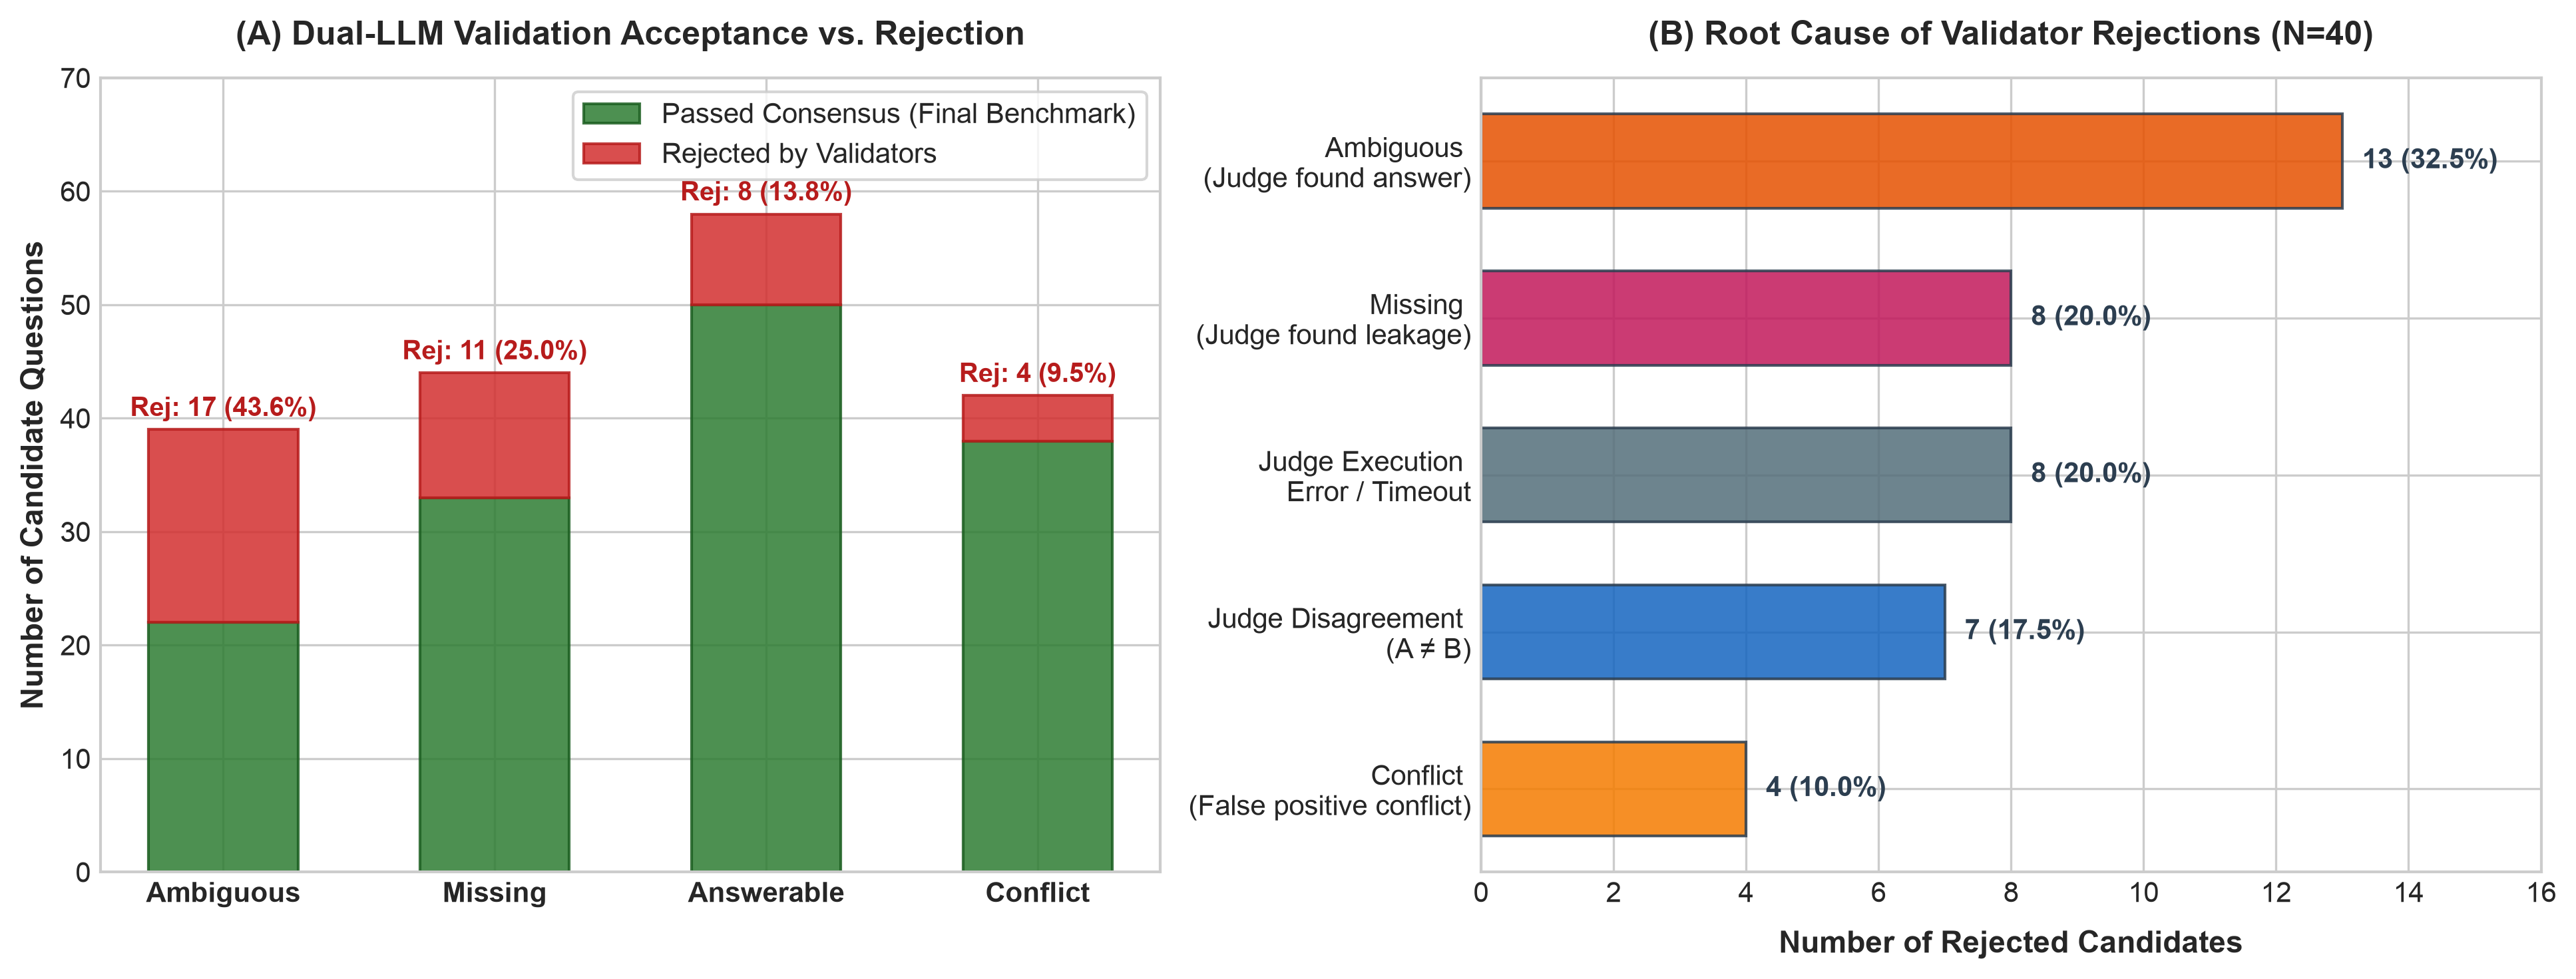
\includegraphics[width=0.6\textwidth]{figures/fig6_validation_rejection_funnel.png}
    \caption{Multi-judge validation funnel illustrating candidate progression and category-level outcomes.}
    \label{fig:validation_funnel}
\end{figure}

\subsubsection{Rejection Rate by Category and Source Filing}
Table~\ref{tab:validation_by_category} details the evaluated, accepted, and rejected counts alongside the primary failure modes for each category.

\begin{table*}[t]
\centering
\small
\caption{Automated validation results and failure modes by intended gold category.}
\label{tab:validation_by_category}
\begin{tabular}{lrrrrp{0.36\textwidth}}
\toprule
\textbf{Category} & \textbf{Evaluated} & \textbf{Accepted} & \textbf{Rejected} & \textbf{Rejection Rate} & \textbf{Primary Failure Mode} \\
\midrule
Ambiguous  & 39  & 22  & 17 & 43.6\% & Under-ambiguity: validators resolved to a single answer. \\
Missing    & 44  & 33  & 11 & 25.0\% & Residual metric leakage remained elsewhere in excerpt. \\
Answerable & 58  & 50  & 8  & 13.8\% & Validator execution timeout or spurious contradiction. \\
Conflict   & 42  & 38  & 4  & 9.5\%  & Disagreement over period alignment or phrasing. \\
\midrule
\textbf{Total} & \textbf{183} & \textbf{143} & \textbf{40} & \textbf{21.9\%} & --- \\
\bottomrule
\end{tabular}
\end{table*}

Table~\ref{tab:validation_by_report} summarizes candidate validation by corporate source filing.

\begin{table}[h]
\centering
\small
\caption{Automated validation breakdown by corporate filing.}
\label{tab:validation_by_report}
\begin{tabular}{lrrrr}
\toprule
\textbf{Report} & \textbf{Evaluated} & \textbf{Accepted} & \textbf{Rejected} & \textbf{Rejection (\%)} \\
\midrule
Coca-Cola   & 59  & 42  & 17 & 28.8\% \\
Caterpillar & 43  & 32  & 11 & 25.6\% \\
Pfizer      & 59  & 52  & 7  & 11.9\% \\
Amazon      & 22  & 17  & 5  & 22.7\% \\
\midrule
\textbf{Total} & \textbf{183} & \textbf{143} & \textbf{40} & \textbf{21.9\%} \\
\bottomrule
\end{tabular}
\end{table}

\subsubsection{Root Causes and Validator Decision Pairs}
The 40 rejected items were categorized into four mutually exclusive root-cause groups (Table~\ref{tab:rejection_causes}) and their specific validator pair combinations (Table~\ref{tab:judge_decision_pairs}).

\begin{table}[h]
\centering
\small
\caption{Root-cause breakdown among the 40 rejected items.}
\label{tab:rejection_causes}
\begin{tabular}{lrr}
\toprule
\textbf{Root cause} & \textbf{Count} & \textbf{Percentage} \\
\midrule
Ambiguity failure               & 16 & 40.0\% \\
Missing-fact leakage            & 9  & 22.5\% \\
Judge execution / format error  & 8  & 20.0\% \\
Conflict disagreement           & 7  & 17.5\% \\
\midrule
\textbf{Total} & \textbf{40} & \textbf{100.0\%} \\
\bottomrule
\end{tabular}
\end{table}

\begin{table*}[t]
\centering
\small
\caption{Detailed validator decision pairs among the 40 rejected items.}
\label{tab:judge_decision_pairs}
\begin{tabular}{lllr}
\toprule
\textbf{Root cause} & \textbf{Validator A (\texttt{gpt-oss:120b})} & \textbf{Validator B (\texttt{nemotron-3-super})} & \textbf{Count} \\
\midrule
Ambiguity failure        & Answerable & Answerable & 7 \\
Ambiguity failure        & Answerable & Ambiguous  & 6 \\
Ambiguity failure        & Answerable & Conflict   & 3 \\
\midrule
Missing-fact leakage     & Answerable & Answerable & 3 \\
Missing-fact leakage     & Answerable & Missing    & 3 \\
Missing-fact leakage     & Missing    & Answerable & 2 \\
Missing-fact leakage     & Ambiguous  & Missing    & 1 \\
\midrule
Execution / format error & Answerable & Error      & 6 \\
Execution / format error & Missing    & Error      & 2 \\
\midrule
Conflict disagreement    & Answerable & Conflict   & 3 \\
Conflict disagreement    & Ambiguous  & Conflict   & 1 \\
Conflict disagreement    & Other edge cases & Other edge cases & 3 \\
\bottomrule
\end{tabular}
\end{table*}

\subsection{Summary of Dataset Fields}
\label{app:dataset_fields}

Table~\ref{tab:dataset_fields} summarizes all primary schema fields recorded in the released benchmark JSONL files. Figure~\ref{fig:dataset_dashboard} provides an integrated dashboard view.

\begin{table}[h]
\centering
\small
\caption{Schema fields recorded in the FinAbstain benchmark.}
\label{tab:dataset_fields}
\begin{tabular}{p{0.32\columnwidth}p{0.62\columnwidth}}
\toprule
\textbf{Field} & \textbf{Description} \\
\midrule
\texttt{gold\_decision}        & Binary ground-truth label (\textit{Answer} or \textit{Abstain}). \\
\texttt{category}             & Fine-grained category (\textit{Answerable}, \textit{Conflict}, \textit{Missing}, \textit{Ambiguous}). \\
\texttt{fact\_type}            & Semantic fact category (\textit{Amount}, \textit{Date}, \textit{Percentage}, \textit{Name}, \textit{Count}, \textit{Other}). \\
\texttt{source\_report}        & Corporate 10-K filing source entity. \\
\texttt{question\_type}        & Syntactic question interrogative form (\textit{What}, \textit{Other}, \textit{How much/many}, \textit{Which}). \\
\texttt{question\_tokens}      & BPE token count of the query under \texttt{cl100k\_base}. \\
\texttt{short\_context\_tokens} & BPE token count of the target excerpt passage. \\
\texttt{full\_context\_tokens}  & BPE token count of the complete padded filing context ($\sim$8,000 tokens). \\
\texttt{evidence\_tokens}      & BPE token count of the ground-truth evidence span. \\
\texttt{answer\_tokens}        & BPE token count of the gold answer string. \\
\texttt{target\_position}      & Normalized position $\tau_i \in [0.0, 1.0]$ of target passage in full context. \\
\bottomrule
\end{tabular}
\end{table}

\begin{figure*}[t]
    \centering
    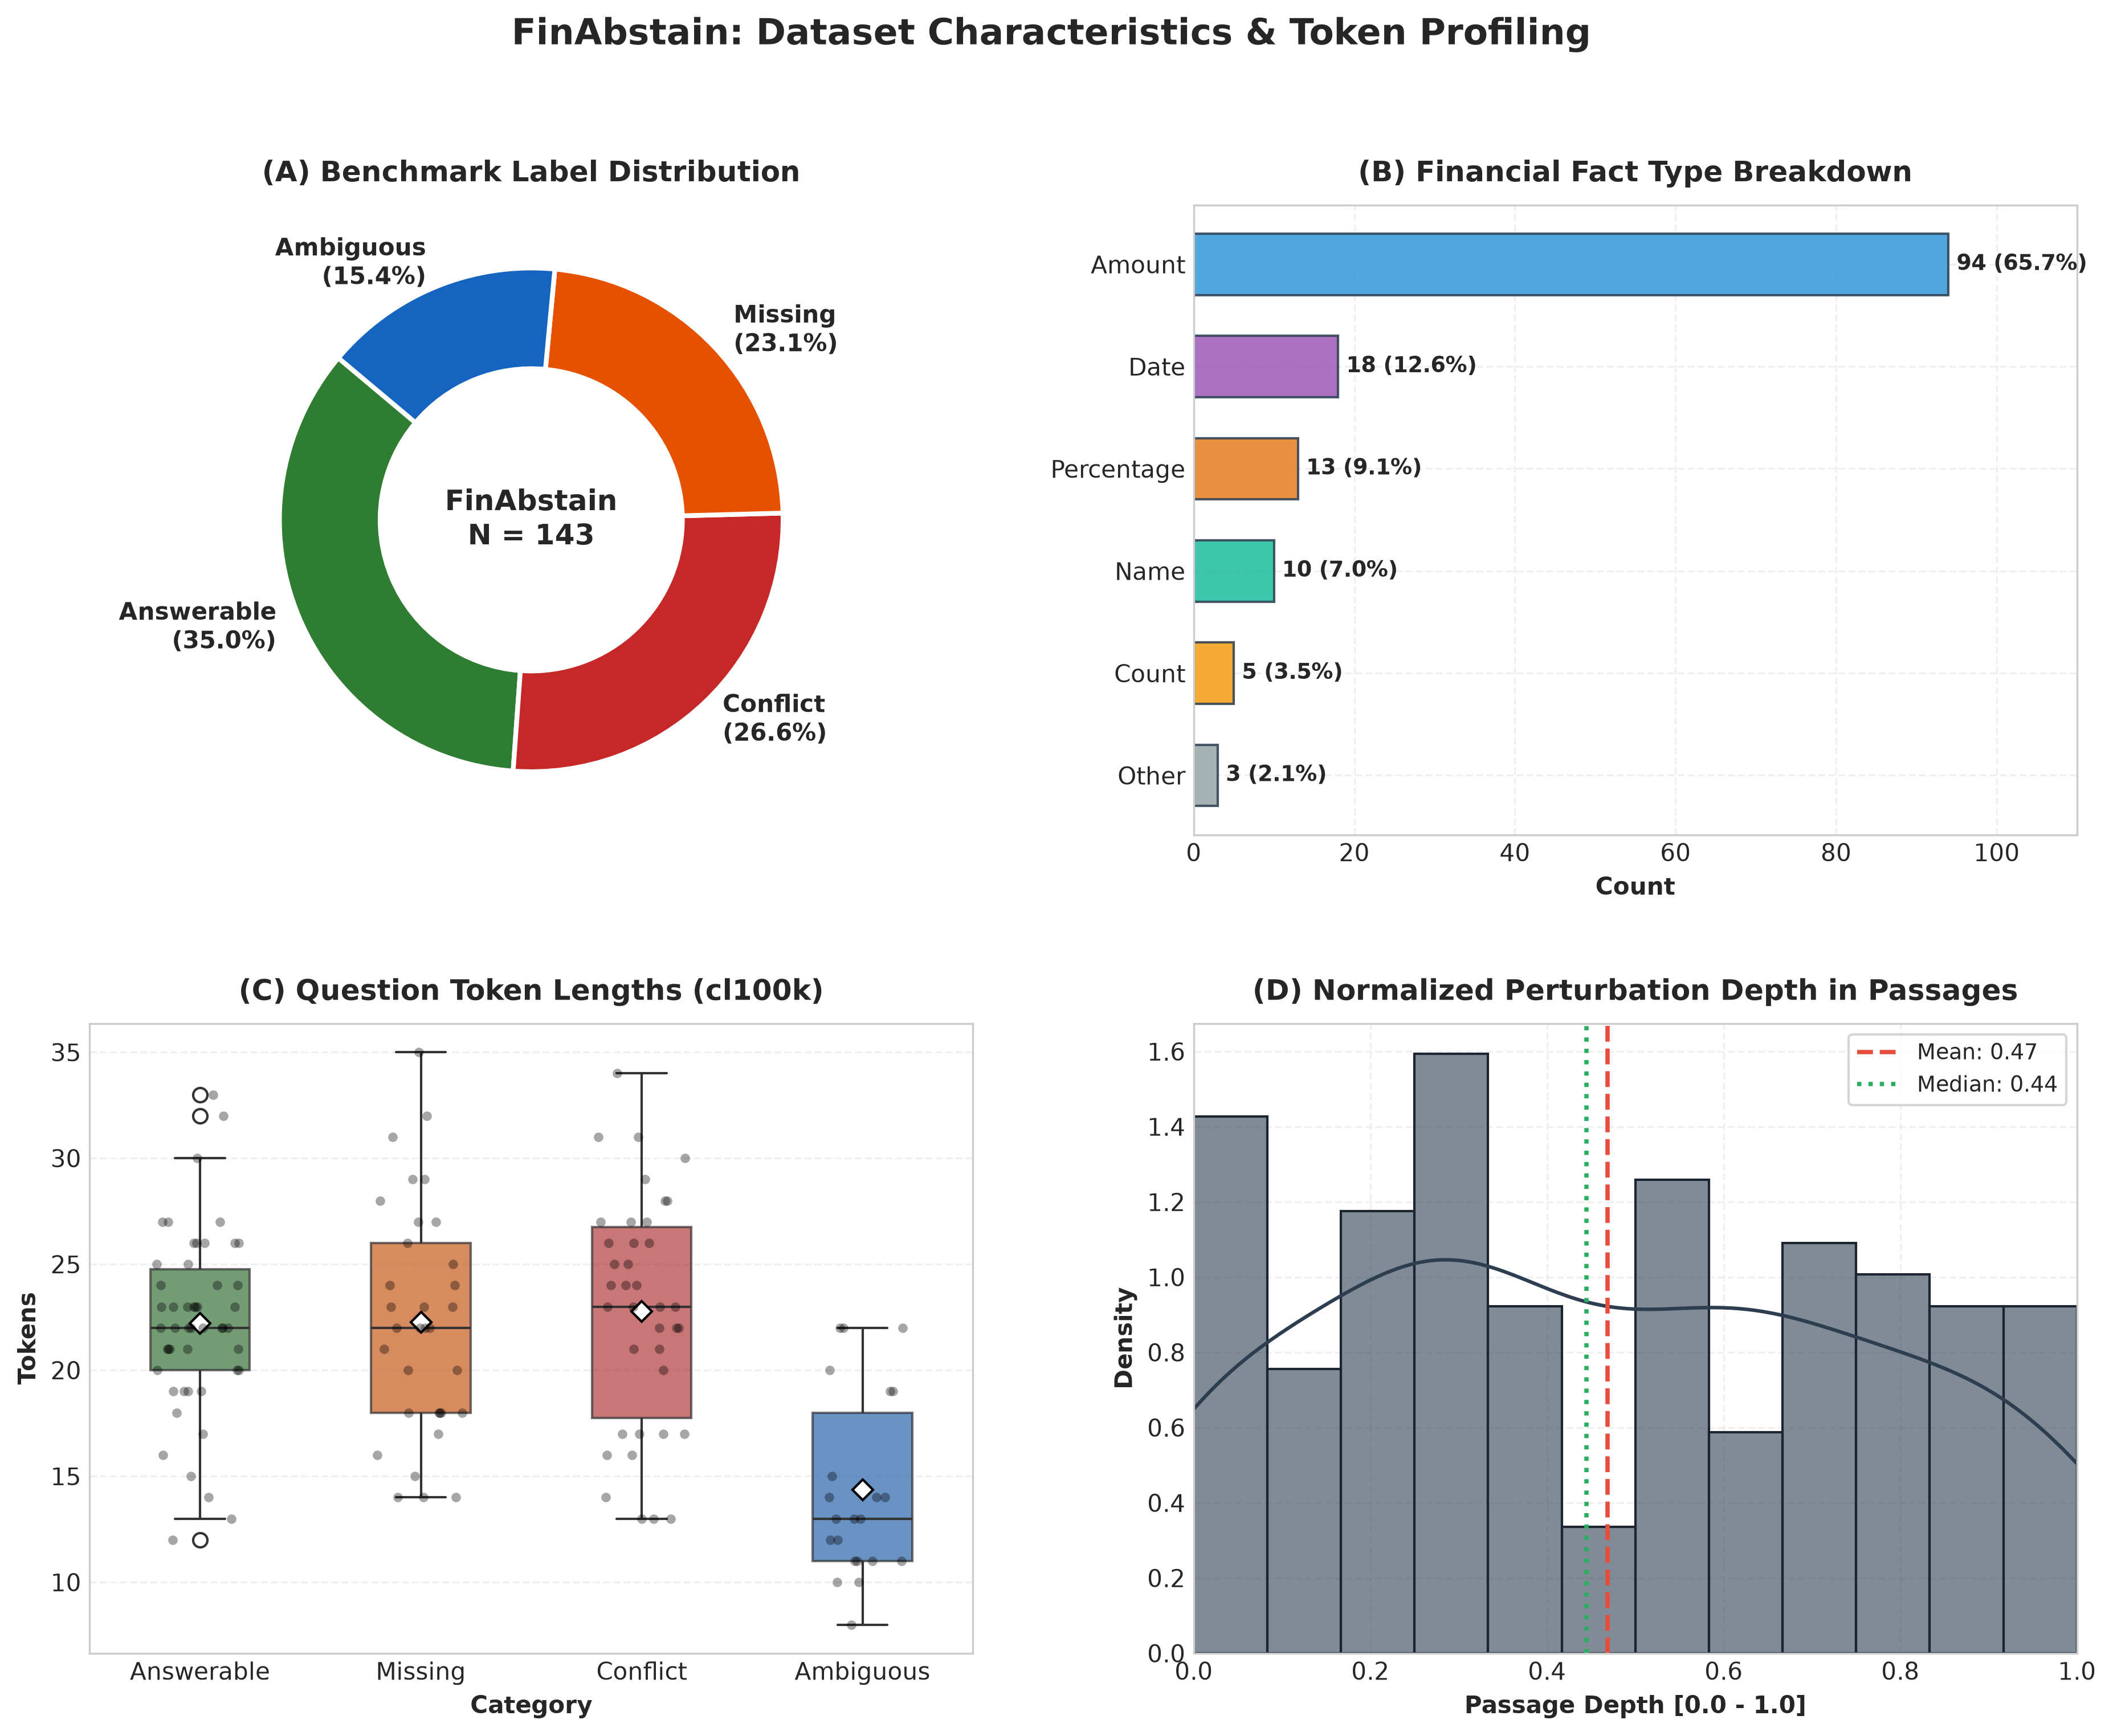
\includegraphics[width=\textwidth]{figures/fig5_dataset_paper_dashboard.png}
    \caption{Integrated benchmark overview: Category distribution, fact types, source filings, token length profiles, and target position depths.}
    \label{fig:dataset_dashboard}
\end{figure*}

\clearpage

\section{Detailed Human Evaluation Results and Annotation Protocol}
\label{app:human_eval_details}

To establish an empirical human performance ceiling, an independent human annotator evaluated 44 stratified items from a blind evaluation pack with no access to ground-truth labels, source filing identifiers, or edit histories.

\subsection{Annotation Protocol and Blinding}
\label{app:human_annotation}
The annotator evaluated the unpadded target passages containing the question and candidate section. To eliminate cognitive bias and prevent shortcut exploitation:
\begin{enumerate}
    \item \textbf{Complete Blinding:} The annotator was never shown the gold category label, underlying edit operations, source filing identifiers, or model validator logs.
    \item \textbf{Anonymization and Rescaling:} Passages contained masked entity names and rescaled financial figures. The annotator was explicitly instructed to rely strictly on the text and ignore external world knowledge regarding real-world corporate filings.
    \item \textbf{Independent Judgment:} The evaluation was completed independently without consultation, ensuring an unbiased assessment of document sufficiency.
\end{enumerate}

\subsection{Operational Definitions and Guidelines}
The annotator read each question, inspected the passage, and selected exactly one of four mutually exclusive operational labels:
\begin{itemize}
    \item \textbf{Answerable:} The passage states exactly one verified value or factual statement that directly and unambiguously answers the query.
    \item \textbf{Missing:} The passage discusses the general topic or business segment of the question, but the specific metric, value, or fact requested is absent.
    \item \textbf{Conflict:} The passage asserts two or more mutually contradictory values for the exact same fact (\textit{i.e.}, identical metric, entity, and fiscal period) with no contextual reconciliations.
    \item \textbf{Ambiguous:} The question lacks key qualifying constraints, resulting in two or more competing, equally valid answers present in the text.
\end{itemize}

\subsection{Systematic Tie-Breaking Rules}
When multiple classifications appeared plausible, the annotator adhered to predefined tie-breaking rules:
\begin{itemize}
    \item \textbf{Conflict vs.\ Ambiguous:} If multiple values correspond to the specific entity and period stated in the question, the item must be labeled \textbf{Conflict}. If the competing values exist because the question left the period, segment, or entity unspecified, it must be labeled \textbf{Ambiguous}.
    \item \textbf{Missing vs.\ Answerable:} If the passage provides a related metric or a figure from an adjacent fiscal period, but not the exact metric queried, the annotator must label \textbf{Missing}.
    \item \textbf{Missing vs.\ Ambiguous:} An item is labeled \textbf{Ambiguous} only if at least two valid answers are concretely present in the passage. If a vague question yields zero candidate answers in the text, it is labeled \textbf{Missing}.
    \item \textbf{Identical Repetitions:} If a metric is repeated identically across different sentences or table summaries, it is labeled \textbf{Answerable} rather than a conflict.
\end{itemize}

\subsection{Quantitative Performance and Reliability Metrics}
Across the 44 audited items, the human annotator achieved a four-class classification accuracy of \textbf{79.55\%} ($35/44$) and a Cohen's $\kappa$ of \textbf{0.7295}, indicating substantial inter-annotator agreement. On the high-level binary decision (\textit{Answer} vs.\ \textit{Abstain}), human accuracy reached \textbf{86.36\%} ($38/44$), with an over-refusal rate of \textbf{0.0\%} (Table~\ref{tab:human_evaluation_detailed}).

\begin{table}[h]
\centering
\small
\caption{Detailed human evaluation breakdown across the 44 audited items. Naturalness denotes the 5-point Likert fluency score.}
\label{tab:human_evaluation_detailed}
\begin{tabular}{lccccc}
\toprule
\textbf{Category} & \textbf{Support} & \textbf{Precision} & \textbf{Recall} & \textbf{F1} & \textbf{Naturalness (1--5)} \\
\midrule
Answerable & 8  & 0.571 & 1.000 & 0.727 & 5.00 $\pm$ 0.00 \\
Missing    & 10 & 1.000 & 0.900 & 0.947 & 4.90 $\pm$ 0.32 \\
Conflict   & 10 & 0.727 & 0.800 & 0.762 & 4.90 $\pm$ 0.32 \\
Ambiguous  & 16 & 1.000 & 0.625 & 0.769 & 4.63 $\pm$ 0.62 \\
\midrule
\textbf{Overall / Macro} & \textbf{44} & \textbf{0.825} & \textbf{0.831} & \textbf{0.801} & \textbf{4.82 $\pm$ 0.44} \\
\bottomrule
\end{tabular}
\end{table}

\begin{table}[h]
\centering
\small
\caption{Full confusion matrix of human predictions vs.\ benchmark gold labels ($N=44$).}
\label{tab:human_confusion}
\begin{tabular}{lccccr}
\toprule
\textbf{Gold Category} & \multicolumn{4}{c}{\textbf{Human Predicted Label}} & \textbf{Total} \\
\cmidrule(lr){2-5}
& \textbf{Answerable} & \textbf{Missing} & \textbf{Conflict} & \textbf{Ambiguous} & \\
\midrule
Answerable & \textbf{8} & 0 & 0 & 0 & 8 \\
Missing    & 1 & \textbf{9} & 0 & 0 & 10 \\
Conflict   & 2 & 0 & \textbf{8} & 0 & 10 \\
Ambiguous  & 3 & 0 & 3 & \textbf{10} & 16 \\
\midrule
\textbf{Total} & 14 & 9 & 11 & 10 & \textbf{44} \\
\bottomrule
\end{tabular}
\end{table}

\subsection{Per-Category Findings: Human vs.\ Language Models}
Comparing human performance against the small open models highlights distinct behavioral characteristics:
\begin{itemize}
    \item \textbf{Answerable Sufficiency (100\% Recall):} The annotator answered all 8 answerable items correctly ($1.000$ recall), matching the high precision of the models while recording zero false refusals.
    \item \textbf{Missing Evidence (90.0\% Recall):} The human recognized missing information in 9 of 10 cases ($F_1 = 0.947$). Only one item was mistakenly answered by synthesizing an adjacent line item.
    \item \textbf{Conflict Recognition (80.0\% Recall vs.\ $\le$10.5\% LLMs):} While the evaluated open models almost completely failed on contradictions ($\le$4 of 38 items), the human annotator recovered 8 of 10 conflict cases ($0.800$ recall), demonstrating that contradiction detection is intuitive for human readers even when models overlook it.
    \item \textbf{Ambiguity Disambiguation (62.5\% Recall vs.\ $\le$9.1\% LLMs):} The human identified 10 of 16 ambiguous items, with precision remaining at $1.000$ (zero false-positive ambiguity claims on other categories).
\end{itemize}

\subsection{Qualitative Benchmark Sanity Ratings}
Alongside label classification, the annotator recorded three qualitative dimensions for each audited sample:
\begin{enumerate}
    \item \textbf{Question Quality (100\% Clear):} Exactly $44/44$ ($100.0\%$) questions were rated as \textit{Clear}. Zero questions were flagged as \textit{Flawed}, verifying that Gemma~4~31B generated grammatically fluent, unambiguous question syntax.
    \item \textbf{Text Fluency and Naturalness ($4.82 / 5.0$):} On a 5-point Likert scale (1 = visibly altered/artificial, 5 = entirely natural SEC text), the benchmark passages averaged $4.82 \pm 0.44$ (median $5.0$). Crucially, perturbed passages scored virtually identically to unmodified passages: Conflict ($4.90$) and Missing ($4.90$) vs.\ Answerable ($5.00$), confirming that the surgical edits did not introduce unnatural artifacts.
    \item \textbf{Annotator Confidence ($2.95 / 3.0$):} Confidence was high across all items (mean $2.95 / 3.0$), indicating clear readability and decisive textual evidence.
\end{enumerate}

\subsection{Detailed Analysis of the 9 Discrepancies}
Review of the 9 items where the annotator disagreed with the benchmark gold label reveals distinct patterns:
\begin{enumerate}
    \item \textbf{Abstention Label Disagreement (3 items):} In 3 ambiguous items, the annotator detected that multiple competing values existed but classified the item as \textit{Conflict} rather than \textit{Ambiguous} (\textit{e.g.}, noting \textit{``Two different types of stock given, not sure which one to use''} or \textit{``\$23M and \$299M, didn't give year in question''}). While counted as an error under strict four-class scoring, both human and benchmark agreed on the high-level policy: \textbf{Abstain}.
    \item \textbf{Implicit Defaults on Ambiguity (3 items):} In 3 ambiguous questions, the annotator answered by adopting an unstated default, picking the consolidated total rather than flagging that individual operating segments were unspecified.
    \item \textbf{Overlooked Contradiction (2 items):} In two conflict items, the human identified the primary reported number but overlooked the conflicting insertion in the following paragraph, mirroring the model's primacy bias.
    \item \textbf{Proxy Answering on Missing (1 item):} In one missing item, the annotator inferred an answer from a closely related footnote disclosure.
\end{enumerate}
Critically, 6 of the 9 disagreements still agreed on the binary decision to abstain, and the human annotator achieved a \textbf{0.0\% over-refusal rate} across all gold Answerable items.

\clearpage

\section{Prompts Used in Benchmark Construction and Evaluation}
\label{app:prompts}

This section lists the verbatim text of all prompts used for downstream model evaluation, question generation, controlled text perturbation, and multi-judge validation.

\subsection{Model Evaluation Prompt}
The following prompt was supplied to all evaluated models (Qwen3.5-9B, Granite-4.1-8B, and Phi-4):

\begin{quote}\small\ttfamily
You are given a financial report excerpt and a question. Decide whether the question can be answered from the text.

Labels:\\
answerable: The text contains exactly one value or fact that answers the question, unambiguously.\\
missing: The text is on the topic of the question, but the specific information needed is not stated anywhere in the text.\\
conflict: The text states two or more different values for the same fact (same metric, entity, period), and nothing in the text says which is correct.\\
ambiguous: The question does not say enough to pick one answer. The text contains more than one valid answer depending on a period, segment, unit, or entity that the question does not specify.

Use only the text. Do not use outside knowledge.\\
Respond with ONLY a JSON object:\\
\{"decision": "answer" or "abstain", "reason": "none" | "missing" | "conflict" | "ambiguous", "answer": "<short answer if decision is answer, else empty string>"\}

If decision is "answer", reason must be "none". If decision is "abstain", reason must be one of missing, conflict, ambiguous.

Text:\\
\{context\}

Question: \{question\}
\end{quote}

\subsection{Question Generation Prompt}
Gemma 4 31B used the following prompt to generate factual questions from selected filing sections:

\begin{quote}\small\ttfamily
You are building a reading-comprehension test from a financial report excerpt.\\
Read the excerpt and write ONE question about a specific fact stated in it.

Rules:\\
- The question must be answerable from the excerpt alone and must uniquely identify the fact (name the metric, the period, and the segment or entity when the excerpt has several).\\
- Prefer numeric facts (amounts, percentages, counts, dates). Avoid yes/no questions.\\
- Do not use phrases like "according to the passage/excerpt/text". Refer to the entity as "the Company".\\
- The question must not contain or hint at the answer.\\
- "answer" is short ($\le$ 12 words), copied or directly derived from the evidence.\\
- "evidence\_span" is copied VERBATIM from the excerpt (one sentence or one table row) and contains the answer.\\
- "fact\_type" is one of: amount, percentage, date, count, name, other.

Return ONLY JSON: \{"question": "...", "answer": "...", "evidence\_span": "...", "fact\_type": "..."\}

Excerpt:\\
\{section\_text\}
\end{quote}

\subsection{Perturbation Prompts}
For candidate unanswerable items, Gemma 4 31B proposed edits under one of the three following prompts.

\subsubsection{Conflict Perturbation Prompt}
\begin{quote}\small\ttfamily
Below is an excerpt, a question, and its answer. Modify the excerpt so that it states TWO different, contradictory values for the same fact (same metric, entity, period), with nothing to reconcile them.

You do this by choosing an anchor line and inserting a single contradictory sentence after it.

Rules:\\
- "anchor" must be a verbatim span (usually a single sentence or line) copied from the excerpt that occurs EXACTLY once.\\
- "inserted\_text" is a short passage ($\le$ 50 words) that will be inserted on a new line immediately after the anchor line.\\
- "conflicting\_value" is the new, alternative value stated in your inserted text for the exact same metric/period/entity as the original answer.\\
- "conflicting\_value" must be plausible and clearly different from the original answer (relative difference $\ge$ 5\% if numeric).\\
- Do NOT use any reconciliation or explanation words in your inserted text, such as: restated, revised, revision, corrected, correction, adjusted, previously, updated, amended, formerly, initially, originally, supersede. The contradiction must be unresolved.\\
- Do NOT modify or delete any existing text from the excerpt.

Return ONLY JSON: \{"anchor": "...", "inserted\_text": "...", "conflicting\_value": "..."\}

Question: \{question\}\\
Original Answer: \{answer\}

Excerpt:\\
\{section\_text\}
\end{quote}

\subsubsection{Missing Evidence Perturbation Prompt}
\begin{quote}\small\ttfamily
Below is an excerpt, a question, and its answer. Remove the information that answers the question.

Return the exact spans to delete. Rules:\\
- Each span must be copied VERBATIM from the excerpt and appear exactly once.\\
- After deleting, the answer value (and any restatement of it, in any format) must not appear anywhere in the excerpt.\\
- The remaining text must stay grammatical and on the same topic; do not delete unrelated content.\\
- Delete as little as possible (typically one sentence or one table row).\\
- Do NOT add any text. Do NOT write that data is missing, withheld, or undisclosed.

Return ONLY JSON: \{"deletions": ["<verbatim span 1>", "..."]\}

Question: \{question\}\\
Answer: \{answer\}

Excerpt:\\
\{section\_text\}
\end{quote}

\subsubsection{Ambiguity Perturbation Prompt}
\begin{quote}\small\ttfamily
Below is an excerpt, a question, and its answer. Make the question ambiguous by inserting a second valid answer into the text along a specific dimension, and removing the specifying detail from the question so that both answers become equally plausible.

Rules:\\
- "blurred\_dimension" must be one of: "period", "segment", "unit", "entity".\\
- "anchor" must be a verbatim span copied from the excerpt that occurs EXACTLY once.\\
- "inserted\_text" is a short passage ($\le$ 50 words) inserted on a new line immediately after the anchor, providing a second value ("distractor\_value") along the chosen dimension such as for a different fiscal year/quarter, a different business segment, or a different entity/unit.\\
- "distractor\_value" must differ from the original answer.\\
- "removed\_from\_question" is a list of words to remove from the original question to make it underspecified. Every word in this list must appear in the original question and must NOT appear in new\_question.\\
- "new\_question" is the resulting ambiguous question. It must NOT introduce new content words beyond those in the original question, and must NOT contain the answer or distractor value.\\
- Do NOT use reconciliation words in inserted\_text: restated, revised, revision, corrected, correction, adjusted, previously, updated, amended, formerly, initially, originally, supersede.

Return ONLY JSON: \{"anchor": "...", "inserted\_text": "...", "distractor\_value": "...", "blurred\_dimension": "...", "new\_question": "...", "removed\_from\_question": [...]\}

Question: \{question\}\\
Original Answer: \{answer\}

Excerpt:\\
\{section\_text\}
\end{quote}

\subsection{Independent Multi-Judge Validation Prompt}
The two validator models (\texttt{gpt-oss:120b} and \texttt{nemotron-3-super}) were prompted independently without access to the ground-truth label:

\begin{quote}\small\ttfamily
You are an expert financial evaluator. Read the financial report excerpt and answer the question, or determine why it cannot be answered.

Rules:\\
1. First decide which category from the taxonomy applies:\\
   - "answerable": The text contains exactly one value or fact that answers the question, unambiguously.\\
   - "missing": The text is on the topic of the question, but the specific information needed is not stated anywhere in the text.\\
   - "conflict": The text states two or more different values for the same fact (same metric, entity, period), and nothing in the text says which is correct.\\
   - "ambiguous": The question does not say enough to pick one answer. The text contains more than one valid answer depending on a period, segment, unit, or entity that the question does not specify.\\
2. If "answerable", provide the concise answer ($\le$ 12 words) in "answer". If not answerable, "answer" should be "none".\\
3. Provide a brief rationale ($\le$ 30 words) explaining your decision.

Return ONLY JSON: \{"label": "answerable|missing|conflict|ambiguous", "answer": "...", "rationale": "..."\}

Question:\\
\{question\}

Excerpt:\\
\{section\_text\}
\end{quote}

\clearpage

\section{Reproducibility Statement}
\label{app:reproducibility}

To ensure complete scientific reproducibility, all evaluation environments, model quantization configurations, and execution scripts are documented below.

\subsection{Evaluation Environment and Hardware}
\begin{itemize}
    \item \textbf{Inference Engine:} All benchmark evaluations were conducted using \href{https://github.com/ggml-org/llama.cpp}{\texttt{llama.cpp}} (release tag \texttt{v0.4.1}).
    \item \textbf{Hardware Infrastructure:} Downstream model inference was executed on an NVIDIA H100 (80\,GB) GPU server under CUDA 12.
    \item \textbf{Model Quantization:} All three evaluated models (\texttt{Qwen3.5-9B}, \texttt{Granite-4.1-8B}, and \texttt{Phi-4-14B}) were evaluated as \texttt{Q8\_0} GGUF quantized binaries to maintain near 16-bit float fidelity while fitting entirely in VRAM.
    \item \textbf{Decoding Hyperparameters:} To eliminate stochasticity, all models were evaluated using deterministic greedy decoding:
    \begin{itemize}
        \item Temperature: $0.0$
        \item Random seed: $42$
        \item Context window limit: $16{,}384$ tokens
        \item Generation limits: 2,048 tokens for Granite-4.1-8B and Phi-4; 200 tokens for Qwen3.5-9B (thinking mode explicitly disabled).
    \end{itemize}
\end{itemize}

\subsection{Dataset Generation and Validation Infrastructure}
\begin{itemize}
    \item \textbf{Local Generation Platform:} The end-to-end dataset generation, controlled text perturbation, and multi-judge validation pipelines were executed locally via \href{https://ollama.com}{\texttt{Ollama}} on an Apple M1 Air (8\,GB unified memory) running macOS version 26.5.2 (25F84).
    \item \textbf{Generation Model:} \texttt{gemma4:31b} served as the primary generator for financial questions, factual answers, and candidate perturbations.
    \item \textbf{Validation Models:} Two independent model checkpoints served as blind validators during Stage~07: \texttt{gpt-oss:120b} (Validator A) and \texttt{nemotron-3-super} (Validator B).
    \item \textbf{Determinism:} All document chunking, filler padding, and section assignments utilized fixed random seeds (Seed $42$ and Seed $2027$) to ensure identical corpus generation upon re-run.
\end{itemize}

\subsection{Statistical Evaluation and Bootstrap Confidence Intervals}
All primary metrics (Reason Macro-F1, Decision Accuracy, Over-Refusal, and Over-Answer rates) report 95\% percentile bootstrap confidence intervals computed using $1{,}000$ resamples over test items with fixed random seed $42$.

\subsection{Artifacts and Code Availability}
The complete benchmark dataset (\texttt{benchmark.jsonl} and \texttt{benchmark\_short.jsonl}), evaluation scripts (\texttt{run\_eval.py}, \texttt{score.py}), and human annotation files are bundled with SHA-256 verification checksums to support independent replication.

\section{AI Use Statement}
\label{app:ai_use}

\begin{enumerate}
    \item \textbf{Benchmark Artifact Generation:} Generative language models were utilized as part of the experimental methodology to construct the benchmark: \texttt{gemma4:31b} proposed questions and candidate perturbations, while \texttt{gpt-oss:120b} and \texttt{nemotron-3-super} served as blind automated validators. All synthetic modifications were governed by deterministic Python verification checks, and final dataset quality was audited via blind human evaluation.
    \item \textbf{Writing and Coding Assistance:} Generative AI assistants were used for preliminary code scaffolding, debugging, formatting LaTeX tables, and grammatical proofreading of draft text. All research design, experimental execution, data analysis, and interpretation were conducted by the authors, who have reviewed all manuscript contents and take full scientific responsibility for the paper.
\end{enumerate}

\bibliographystyle{plainnat}
\bibliography{references}

\end{document}
